% !TeX root = ../economia.tex
\chapter{Contabilità Interna}
La contabilità interna nasce con due obiettivi fondamentali:
supportare l’elaborazione dei dati di contabilità esterna (\emph{valore scorte})
e fornire una gamma di \emph{informazioni dettagliate} (ai fini decisionali e del
controllo di gestione), \emph{non reperibili nei dati di contabilità generale}.

Tali informazioni possono essere relative a:
\begin{itemize}
    \item prodotti (costo di prodotto, analisi make or buy\dots)
    \item unità organizzative (valutazioni di efficienza, produttività\dots)
\end{itemize}

In particolare, le informazioni di contabilità interna sono utilizzate per:
\begin{itemize}
    \item valorizzazione delle scorte (obiettivo comune ad analisi di contabilità
    esterna ed interna)
    \item analisi gestionali, sia di breve che di lungo periodo, finalizzate alla
    pianificazione e al controllo delle attività:
    \begin{itemize}
        \item Supporto all’elaborazione del budget d’impresa
        \item Analisi di profittabilità
        \item Introduzione/eliminazione codici di prodotto
        \item Efficienza centri produttivi o di servizio;
        \item Scelte di esternalizzazione (outsourcing);
        \item Decisioni tattiche di mix, pricing, ecc.
    \end{itemize}
    \item valutazione del personale (legami col sistema di incentivi)
\end{itemize}

\section{Analisi dei costi}
Le voci di \gls{costo} elementari possono essere \emph{classificate} secondo diversi criteri,
in relazione allo specifico obiettivo che ci si prefigge nell’analisi.

Un sistema di \emph{Cost Accounting} ha come obiettivo l’allocazione
dei costi agli oggetti di costo:
\begin{itemize}
    \item Prodotti
    \item Servizi
    \item Unità Organizzative
\end{itemize}

\subsection{Ammortamento}
Immobili, impianti, attrezzature e macchinari sono beni aventi utilità
pluriennale. È necessario quindi porsi il problema di determinare un loro \emph{\gls{costo}}
annuo, indipendentemente dal momento in cui si effettua l’acquisto.
Questo \emph{costo} tiene conto del fatto che io sto \emph{consumando} il bene
attraverso il suo utilizzo.

In contabilità interna, il \emph{costo} annuo di un bene ad utilità pluriennale
viene chiamato \emph{\gls{ammortamento}}.

\paragraph{Determinare l'ammortamento} 
\begin{equation*}
    \text{Ammortamento} = \frac{\text{\Gls{costo} del bene}}{\text{\Gls{vitautile}}}
\end{equation*}

\subsection{Classificazioni delle voci di costo}

\subsubsection{Costi diretti/indiretti}
Un costo si dice \emph{diretto} se può essere attribuito \emph{in modo univoco e
inequivocabile} ad un determinato oggetto di costo (prodotto o
servizio).
Tutte le restanti voci di costo vanno considerate come costi \emph{indiretti} (o
overhead).

La presenza di costi indiretti comporta il \emph{problema} della loro
\emph{allocazione}, nel caso in cui si voglia attribuirli ai prodotti.

\subsubsection{Costi variabili/fissi}
Un costo si dice \emph{variabile} quando varia in modo direttamente
proporzionale al variare del volume di produzione. Un costo si dice \emph{fisso}
quando non varia al variare del volume di produzione.

L'identificazione del costo fisso/variabile richiede la definizione
dei seguenti elementi:
\begin{itemize}
    \item orizzonte temporale di riferimento
    \item volume operativo
\end{itemize}

\subsubsection{Costi di prodotto}
Valore delle risorse utilizzate per la realizzazione
di un determinato prodotto/servizio. Tipicamente sono:

\paragraph{Costi di materiali diretti (MD)}
Materie prime, componenti, semilavorati
associabili direttamente alla produzione di un determinato
prodotto/servizio\dots

\paragraph{Costi del lavoro diretto (LD)}
Relativi agli addetti alle operazioni di
trasformazione fisica degli input e di assemblaggio dei componenti

\paragraph{Costi indiretti di produzione (OVH)}
Costi non imputabili direttamente ai singoli prodotti, sebbene associabili
all’attività produttiva nel suo complesso

\subsubsection{Costi di periodo}
Valore delle risorse impiegate in attività non
associabili alla realizzazione di un prodotto/servizio secondo un nesso
di causalità (ovvero non direttamente associabili alle operazioni di
trasformazione fisica dell’input in output). Tipicamente sono:

\paragraph{Costi amministrativi}
Personale, altri costi amministrazione

\paragraph{Spese generali}
Stipendi di dirigenti e impiegati uffici centrali,
ammortamenti di macchinari, attrezzature, fabbricati non industriali,
spese generali di sede (telefono, missioni\dots), assicurazioni di
dipendenti uffici e fabbricati non industriali\dots

\paragraph{Spese di vendita}
Stipendi e spese di viaggio degli agenti di
vendita interni, ammortamento, assicurazioni, spese operative o di
manutenzione automezzi venditori/distributori\dots

\paragraph{Spese discrezionali}
Pubblicità, promozione, partecipazione a
fiere, corsi di formazione e aggiornamento, costi legali, attività
culturali e ricreative\dots

\subsubsection{Costi inventariabili/non inventariabili}
La distinzione tra costi di prodotto e costi di periodo è fondamentale
per la valorizzazione delle scorte.

I \emph{costi di prodotto} sono anche detti \emph{costi inventariabili} perchè
vengono ``incorporati'' nel valore delle scorte, e quindi vanno a costituire il
\emph{valore} di magazzino di una impresa.

Al contrario i \emph{costi di periodo} sono anche detti \emph{non inventariabili},
ovvero non contribuiscono a determinare il \emph{valore} del magazzino.

\vspace{1em}
\begin{tabular}{|c|c|c|c|}
    \hline
    \multirow{2}{*}{Costi di \textsc{periodo}} & \multicolumn{3}{c|}{Costi di \textsc{prodotto}}\\
    \cline{2-4}
    & Materiali Diretti & Lavoro Diretto & Overhead di produzione \\
    \hline
\end{tabular}

\subsubsection{Costi storici}
Il costo storico è quello rilevato a consuntivo, cioè dei beni consumati anzichè prodotti.

Servono per la consuntivazione e l’allocazione dei costi effettivamente
sostenuti dall’impresa in un determinato intervallo, e sono fondamentali per la
determinazione dei risultati economici e per la valorizzazione delle scorte

\subsubsection{Costi standard}
Il costo standard è il costo ``teorico, ingegneristico, ottenibile dall’impresa in condizioni
di normale funzionamento''.

\begin{itemize}
    \item ``costo teorico [\dots] ottenibile'': è definito ex-ante, sulla base di una serie di
    informazioni (distinta base, cicli di lavorazione, prezzi dei fattori), e rappresenta
    generalmente l’obiettivo di riferimento per la successiva analisi degli scostamenti
    a consuntivo.
    \item ``condizioni di normale funzionamento'': sono esclusi eventi straordinari che
    modifichino in modo rilevante le \emph{condizioni al contorno}.
\end{itemize}

Si possono definire tre tipi di costi standard, in base al livello di efficienza richiesto:
\begin{itemize}
    \item Costo standard \emph{ideale}
    \item Costo standard \emph{raggiungibile}
    \item Costo standard \emph{normale}
\end{itemize}

Sono utilizzati per la stima dei costi che l’impresa
dovrà sostenere nel futuro, e sono particolarmente utili per l’elaborazione dei budget
operativi e per alcune scelte fondamentali in sede di pianificazione (\emph{mix}, \emph{make or buy}\dots)

\subsubsection{Costi evitabili/non evitabili}
Si definiscono \emph{costi evitabili} quelli influenzati da una specifica decisione, e variano in base a:
\begin{itemize}
    \item L'orizzonte temporale di riferimento
    \item La tecnologia considerata 
\end{itemize}

Si definiscono \emph{costi non evitabili} quelli non influenzati da una specifica decisione.

Tale distinzione è rilevante solo nel \emph{decision-making} (in particolare nelle analisi di
breve periodo).

\subsection{Curva di costo}

\subsubsection{Economie di scala}

\begin{equation*}
    C(Q) < Q(Q_1) + C(Q_2) \quad
    \text{dove} \quad Q_1 + Q_2 = Q
\end{equation*}
\begin{figure}[h]
    \centering
    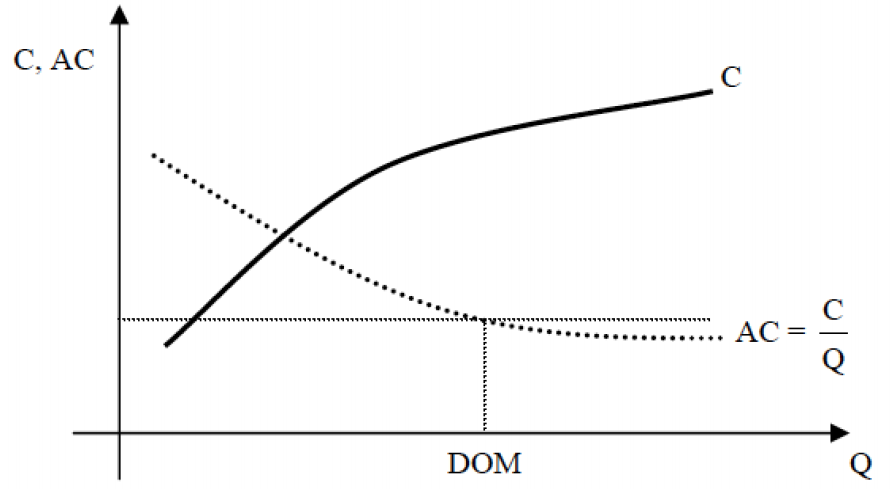
\includegraphics[width=7cm]{economia_di_scala.png}
    \caption{Le economie di scala: costo totale $C$ e costo medio $AC$ in
    funzione di $Q$}
\end{figure}

\subsubsection{Economie di scopo}
Il costo della produzione congiunta di due prodotti ($x$, $y$) sarà inferiore alla
somma della produzione disgiunta di ciascuno di essi.
\begin{equation*}
    C(x,0) + C(0, y) > C(x,y)
\end{equation*}

\subsubsection{Economie di esperienza/apprendimento}
\begin{figure}[h]
    \centering
    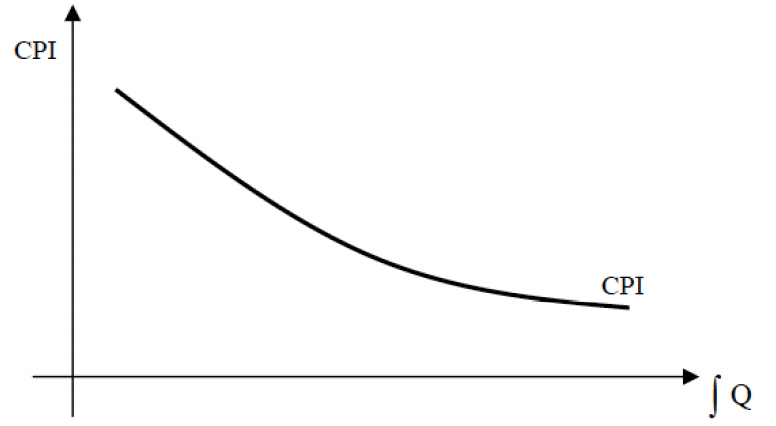
\includegraphics[width=7cm]{economia_di_apprendimento.png}
    \caption{Le economie di apprendimento: costo unitario $CPI$ in funzione della quantità
    di produzione cumulata}
\end{figure}

\subsection{Calcolo del costo pieno industriale}
Al fine di stabilire il costo di realizzazione di un prodotto è necessario
calcolarne il \gls{CPI} (costo pieno industriale), cioè l'insieme dei costi dei materiali
diretti, del lavoro diretto e dell'\emph{overhead} di produzione.

Il calcolo dei costi pieni di prodotto presenta una significativa difficoltà:
quella di attribuire una quota dei costi indiretti ad uno specifico prodotto.

\subsection{Logiche di valorizzazione delle scorte}

\paragraph{FIFO} Le materie prime in ingresso finiscono in magazzino finchè
tutte le altre più vecchie sono state utilizzate.

\paragraph{LIFO} Le materie prime in ingresso sono le prime ad essere utilizzate.

\subsection{Product costing}
L’attribuzione delle voci di costo ai prodotti può avvenire con modalità
distinte, a seconda dello specifico metodo di product costing utilizzato.
In particolare tali metodi si distinguono sulla base della \emph{modalità di
allocazione dei costi indiretti} che può essere:
\begin{itemize}
    \item \textbf{proporzionale}: si attribuiscono al singolo prodotto delle quote di
    costi indiretti proporzionalmente al consumo di una determinata
    risorsa, detta \emph{base di allocazione}, da parte di quel prodotto.
    \item \textbf{causale}: si attribuiscono al singolo prodotto i costi relativi alle
    risorse \emph{indirette} specificamente consumate da quel prodotto.
\end{itemize}

\paragraph{Metodi di product costing}\quad

\vspace{1em}
\begin{tabular}{|l|l|l|l|}
    \hline\grayrow
    \textbf{Metodo} & \textbf{MD} & \textbf{LD} & \textbf{OVH}\\
    \hline
    Job Order Costing (\textsc{joc}) & Causale & Causale & Proporzionale\\
    \hline
    Process Costing (\textsc{pc}) & Proporzionale & Proporzionale & Proporzionale\\
    \hline
    Activity Based Costing (\textsc{abc}) & Causale & Causale & Causale\\
    \hline
\end{tabular}

\subsection{Job Order Costing (JOC)}
È utilizzato in organizzazioni il cui output (in termini di prodotti) è
\emph{chiaramente quantificabile in unità/lotti}.

Il \textsc{JOC} si è sviluppato storicamente nei settori dell'edilizia,
della stampa, dell'aeronautica e nell'impiantistica, ma 
può essere utilizzato anche in organizzazioni non manifatturiere.

\subsubsection{Job order record (o job-cost sheet)}
Il documento fondamentale del job order costing è il \emph{job order record}
o \emph{job-cost sheet}: si tratta della scheda in cui vengono annotate tutte
le voci di costo associabili al job durante la sua lavorazione (nel
momento in cui tali costi sono sostenuti). L'aspetto di un job-cost sheet è la seguente:

\vspace{1em}
\begin{tabular}{l l l}
    Job N. \dots & Data inizio \dots & Cliente \dots \\
    Cod. \dots & Data termine \dots & Priorità \dots \\
\end{tabular}
\newline
\vspace{1em}
\begin{tabular}{|c|c|c|c|c|c|c|c|c|c|c|c|c|}
    \hline
    \multicolumn{4}{|c|}{Materiali Diretti} & \multicolumn{4}{c}{Lavoro Diretto} & \multicolumn{4}{|c|}{Overhead} & \textsc{tot} \\
    \hline
    Data & Rif. & Q.tà & Valore & Data & Rif. & Q.tà & Valore & Data & Rif. &  & Valore & \\
    \hline
\end{tabular}


Quando si utilizza il \textsc{joc}, le voci relative ai costi diretti (\textsc{md} e \textsc{ld})
vengono \emph{caricate} sui job order record in tempo reale e sono quindi
disponibili e direttamente (e univocamente) associate al lotto/prodotto.

\paragraph{Allocazione dei costi indiretti} consiste di tre fasi:
\begin{enumerate}
    \item determinazione delle voci di costo indiretto (overhead) da
    allocare
    \item scelta della base di allocazione (indicatore del consumo delle
    risorse)
    \item allocazione degli overhead ai diversi prodotti
\end{enumerate}

\paragraph{Coefficiente di allocazione}
\begin{equation*}
    K = \frac{\text{OH totali}}{\text{Base di allocazione totale}}
\end{equation*}

Al $j$-esimo \emph{job} vengono allocati costi indiretti $CI$ pari a:
\begin{equation*}
    CI = K \times BA_j
\end{equation*}

dove $BA$ rappresenta l'utilizzo della \emph{base di allocazione} da parte del $j$-esimo job.

\subsection{Process costing (PC)}
Il \emph{process costing} è particolarmente indicato nel caso di sistemi
produttivi caratterizzati da flussi continui attraverso una serie di fasi
di lavorazione condivise dai vari prodotti.
Nel process costing, a differenza del \textsc{joc}, non c'è un’attribuzione
progressiva delle singole voci di costo ai job-order record: al
contrario, esse sono inizialmente indifferenziate e sommate, per
essere quindi distribuite ad intervalli regolari di tempo sui vari
prodotti realizzati, sulla base del volume di output.

\subsubsection{Calcolo del costo di prodotto} Sotto le seguente ipotesi:
\begin{itemize}
    \item Produzione monoprodotto
    \item Produzione monoreparto
    \item Assenza di \textsc{wip} iniziale e finale
    \item Unico pool di costi (MD $+$ LD $+$ OVH)
\end{itemize}
il calcolo del \emph{costo unitario del prodotto} realizzato in un determinato
periodo è molto semplice:
\begin{equation*}
    C_u = \frac{C_{\text{tot}}}{Q} \qquad
    \text{dove} \qquad C_\text{tot} = C_\text{MD} + C_\text{LD} + C_\text{OVH}
\end{equation*}

Per allocare i costi tra \textsc{wip} e produzione completata, si introducono i concetti
di \emph{grado di completamento} e di \emph{unità equivalente}.

\paragraph{Grado di completamento}
indica il grado di completamento del WIP, calcolato in termini di percentuale di
risorse utilizzate in rapporto al totale di input necessari per la produzione di
quel prodotto (si tratta comunque di un rapporto tra valori monetari/risorse
utilizzate basato su valori storici).

\paragraph{Unità equivalenti}
unità di \emph{prodotti finiti} che l’impresa
avrebbe potuto realizzare se avesse realizzato solamente unità complete. In
pratica, si esprime l’output in termini di unità equivalenti di prodotti finiti.

\begin{equation*}
    \text{UE (unità equivalenti)} = Q_c + \text{WIP}_f \times \text{Grado di completamento}
\end{equation*}
\begin{equation*}
    C_\text{UE} = \frac{C_\text{TOT}}{\text{UE}}
\end{equation*}
\begin{equation*}
    C_\text{PF} = C_\text{UE}
\end{equation*}
\begin{equation*}
    \text{Valore \textsc{WIP}} = C_\text{UE} \times \text{WIP} \times \text{Grado di completamento}
\end{equation*}

Se ci fossero anche \textsc{wip} \emph{iniziali} con il loro grado di completamento e il loro
costo $C_\text{WIP,i}$, usando la logica FIFO otterremo:

\begin{equation*}
    \text{UE} = Q_c + \text{WIP}_f \times \text{Grado di completamento \emph{finale}} -
    \text{WIP}_i \times \text{Grado di completamento \emph{iniziale}}
\end{equation*}
\begin{equation*}
    C_\text{UE} = \frac{C_\text{TOT}}{\text{UE}}
\end{equation*}
\begin{equation*}
    C_\text{PF} = C_\text{TOT} + (C_\text{WIP,i} - C_\text{WIP,f}) + C_\text{UE} \times
    (1 - \text{Grado di completezza \emph{iniziale}}) \times \text{WIP}_i + C_\text{UE} \times (Q_c - Q_i)
\end{equation*}
\begin{equation*}
    \text{Valore \textsc{WIP}} = C_\text{UE} \times \text{WIP}_f \times \text{Grado di completamento}
\end{equation*}

\subsubsection{Produzione multiprodotto}
Raramente in un reparto si produce un solo tipo di prodotto: in
particolare, i processi produttivi cui si addice il process costing sono
spesso caratterizzati dalla presenza di \emph{by-product}, che si ottengono
interrompendo il processo a stadi intermedi.

Per l’allocazione dei costi è necessario conoscere il \emph{rapporto tra il
consumo di risorse di ogni singolo prodotto}.

Si introduce il \emph{coefficiente di equivalenza tra prodotti}, assumendo
uno di essi come prodotto di riferimento

\paragraph{Unità equivalenti} unità di \emph{prodotti finiti}
che l’impresa avrebbe potuto realizzare se avesse realizzato
solamente unità complete di un solo tipo di prodotto (il prodotto di
riferimento). In pratica, si esprime l’output in termini di unità
equivalenti di PF del prodotto di riferimento.

\begin{equation*}
    \text{UE} = Q_c + \text{WIP}_f \times \text{Coefficiente di equivalenza}
\end{equation*}
\begin{equation*}
    C_\text{UE} = \frac{C_\text{TOT}}{\text{UE}}
\end{equation*}
\begin{equation*}
    C_\text{PF} = C_\text{UE}
\end{equation*}
\begin{equation*}
    \text{Valore \textsc{WIP}} = C_\text{UE} \times \text{WIP}_f \times \text{Grado di completamento} \times \text{Coefficiente di equivalenza}
\end{equation*}

\subsection{Crisi dei metodi di costing tradizionali}
Tutte le metodologie prevedono un’allocazione dei costi
comuni \emph{proporzionale a qualche grandezza} legata ai \emph{volumi di
produzione}. Fattori come la crescente \emph{complessità delle attività},
il numero e l’importanza crescente di attività non legate ai \emph{volumi} e
il peso crescente degli \emph{overhead} sul totale dei costi d’impresa
mettono in crisi questo tipo di criteri, e rendono necessarie metodologie \emph{più
appropriate}.

\subsection{Activity based costing (ABC)}
Introduce il concetto di attività, come elemento di collegamento/nesso causale
tra le \emph{risorse} (e i costi associati) e i \emph{prodotti}.

\subsubsection{Step logici}
\begin{enumerate}
    \item Identificare le attività che determinano il consumo delle risorse e il
    loro peso relativo (in termini di consumo)
    \item Calcolare i costi delle attività sulla base del rispettivo consumo di
    risorse (attribuendo/allocando i costi delle risorse tramite opportuni
    \emph{resource driver})
    \item Identificare gli \emph{activity driver} per ciascuna attività, ossia le
    grandezze che spiegano l’utilizzo di ciascuna attività da parte dei
    prodotti
    \item Allocare i costi delle attività ai prodotti tramite gli \emph{activity driver}
    identificati
\end{enumerate}